\documentclass[../tp2.tex]{subfiles}

\begin{document}

A tecnologia \textit{Multi-Level Security} refere-se a um esquema de segurança que impõe o \textit{Mandatory Access Model} Bell-La Padula. A aplicação de um sistema informático para processar informações com sensibilidades diferentes, isto é, a diferentes níveis de segurança (Figura \ref{fig:niveis}), permite o acesso simultâneo de utilizadores com diferentes autorizações de segurança e necessidades de conhecimento e impede que os utilizadores obtenham acesso a informações para as quais não têm autorização.\par

\begin{figure}[H]
\centering
\captionsetup{justification=centering,margin=2cm}
\centerline{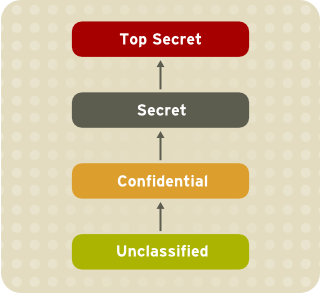
\includegraphics[scale=0.45]{../imagens/niveis.png}}
\caption{Níveis de segurança.}
\label{fig:niveis}
\end{figure}

As regras de acesso MLS são sempre combinadas com permissões de acesso convencionais (permissões de ficheiros). Por exemplo, se um utilizador com um nível de segurança de \textit{``Secret''} usa o \textit{Discretionary Access Control} (DAC) para bloquear o acesso a um ficheiro para outros utilizadores, isso também bloqueia o acesso a utilizadores com um nível de segurança de \textit{``Top Secret''}. É importante lembrar que as regras de política do SELinux MLS são verificadas após as regras do DAC. Uma autorização de segurança mais elevada não dá automaticamente permissão para procurar arbitrariamente um sistema de ficheiros.\par

Os utilizadores com autorizações de nível superior não adquirem automaticamente direitos administrativos aos sistemas de vários níveis. Embora eles possam ter acesso a todas as informações no computador, isso é diferente de ter direitos administrativos.\par 

As seguintes etapas são utilizadas para habilitar a política SELinux MLS no sistema, é um serviço bastante complexo daí ser apenas fornecida uma breve explicação de como este é configurado de forma a funcionar num sistema Linux.\par 

\begin{enumerate}
\item Instalação do pacote selinux-policy-mls.\par
\begin{figure}[H]
\centering
\captionsetup{justification=centering,margin=2cm}
\centerline{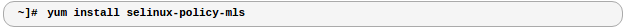
\includegraphics[scale=0.7]{../imagens/install.png}}
\end{figure}


\item Antes da diretiva MLS ser habilitada, cada ficheiro no sistema deve ser classificado com um rótulo MLS de acordo com o modelo BLP elaborado acima. Depois do sistema de ficheiros ser classificado, domínios confinados podem ter acesso negado, o que pode impedir o sistema de iniciar corretamente. Para evitar que isso aconteça, é necessário a configuração \code{SELINUX = permissivo} no ficheiro \code{/etc/selinux/config}. Além disso, é também necessário a habilitação da diretiva MLS configurando \code{SELINUXTYPE = mls}.\par
\begin{figure}[H]
\centering
\captionsetup{justification=centering,margin=2cm}
\centerline{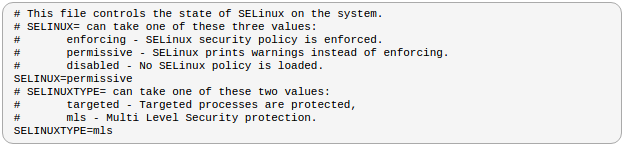
\includegraphics[scale=0.7]{../imagens/config.png}}
\end{figure}

\item Configuração do SELinux em execução no modo permissivo.\par
\begin{figure}[H]
\centering
\captionsetup{justification=centering,margin=2cm}
\centerline{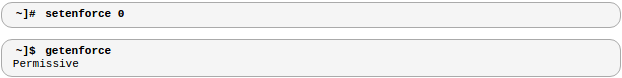
\includegraphics[scale=0.7]{../imagens/permissivo.png}}
\end{figure}

\item Criação de um ficheiro \textit{.autorelabel} na diretoria de raiz para garantir que os ficheiros sejam classificados na reinicialização seguinte do sistema.\par
\begin{figure}[H]
\centering
\captionsetup{justification=centering,margin=2cm}
\centerline{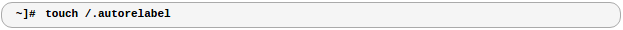
\includegraphics[scale=0.7]{../imagens/auto.png}}
\end{figure}

\item Reinicialização  do sistema, durante a próxima inicialização, todos os sistemas de ficheiros serão classificados de acordo com a política MLS. O processo classifica todos os ficheiros com um contexto SELinux apropriado.\par
\begin{figure}[H]
\centering
\captionsetup{justification=centering,margin=2cm}
\centerline{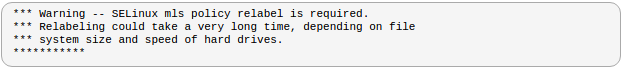
\includegraphics[scale=0.7]{../imagens/reclassificacao.png}}
\end{figure}
Os caracteres $``*"$ na linha inferior representa 1000 ficheiros que foram classificados. No exemplo acima, onze caracteres representam 11000 ficheiros já classificados. O tempo necessário para esta operação depende do número de ficheiros no sistema e da velocidade das unidades de disco rígido. Em sistemas modernos, esse processo pode levar apenas 10 minutos. Quando o processo de classificação terminar, o sistema será reinicializado automaticamente.\par

\item No modo permissivo, a política SELinux não é aplicada, mas as tentativas de acesso negadas ainda são registadas. Antes de mudar para o modo de \textit{``enforcing''}, como \textit{root}, é necessário a execução do seguinte comando para confirmar que o SELinux não negou ações durante a última inicialização. Se o SELinux não negou ações durante o último arranque, este comando não retorna nenhuma saída.\par
\begin{figure}[H]
\centering
\captionsetup{justification=centering,margin=2cm}
\centerline{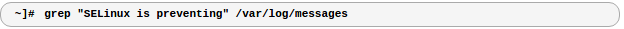
\includegraphics[scale=0.7]{../imagens/iniciar.png}}
\end{figure}

\item Se não houver mensagens de negação no ficheiro \code{/var/log/messages}, ou se tiver resolvido todas as recusas existentes, é necessário a configuração do \code{SELINUX = enforcing} no ficheiro \code{/etc/selinux/config}.\par
\begin{figure}[H]
\centering
\captionsetup{justification=centering,margin=2cm}
\centerline{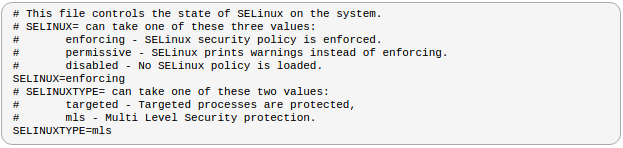
\includegraphics[scale=0.7]{../imagens/enforce.png}}
\end{figure}

\item Por fim, é necessário a reinicialização do sistema, verificando que o SELinux está em execução no modo de \textit{``enforcing''} e a política MLS está habilitada.\par
\begin{figure}[H]
\centering
\captionsetup{justification=centering,margin=2cm}
\centerline{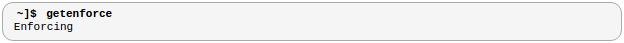
\includegraphics[scale=0.7]{../imagens/enforceEnable.png}}
\end{figure}
\begin{figure}[H]
\centering
\captionsetup{justification=centering,margin=2cm}
\centerline{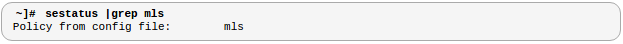
\includegraphics[scale=0.7]{../imagens/mls.png}}
\end{figure}
\end{enumerate}

As seguintes etapas são utilizadas para criar um novo utilizador com um intervalo MLS específico.\par

\begin{enumerate}
\item Criação de um novo utilizador usando o comando \textit{useradd} e mapeamento deste para um utilizador SELinux existente, neste caso, \textit{user\_u}.\par 

\begin{figure}[H]
\centering
\captionsetup{justification=centering,margin=2cm}
\centerline{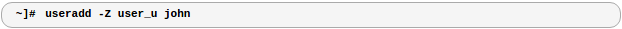
\includegraphics[scale=0.7]{../imagens/adduser.png}}
\end{figure}

\item Atribuição de uma palavra passe ao utilizador recém-criado.\par 
\begin{figure}[H]
\centering
\captionsetup{justification=centering,margin=2cm}
\centerline{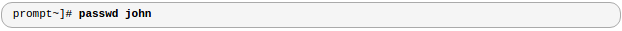
\includegraphics[scale=0.7]{../imagens/pass.png}}
\end{figure}

\item Execução do seguinte comando como \textit{root} para visualizar o mapeamento entre os utilizadores do SELinux e do Linux, o resultado deve ser parecido com o seguinte.
\begin{figure}[H]
\centering
\captionsetup{justification=centering,margin=2cm}
\centerline{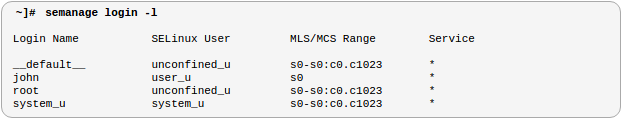
\includegraphics[scale=0.7]{../imagens/users.png}}
\end{figure}

\item Definição de um intervalo específico para o utilizador.\par 
\begin{figure}[H]
\centering
\captionsetup{justification=centering,margin=2cm}
\centerline{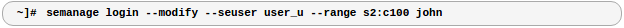
\includegraphics[scale=0.7]{../imagens/range.png}}
\end{figure}

\item Visualização novamente o mapeamento entre os utilizadores do SELinux e do Linux, agora o utilizador tem um intervalo MLS específico definido.\par 
\begin{figure}[H]
\centering
\captionsetup{justification=centering,margin=2cm}
\centerline{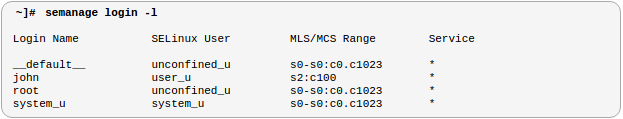
\includegraphics[scale=0.7]{../imagens/definido.png}}
\end{figure}

\item Correção do rótulo na diretoria pessoal do utilizador executando o seguinte comando.\par
\begin{figure}[H]
\centering
\captionsetup{justification=centering,margin=2cm}
\centerline{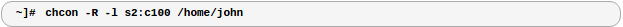
\includegraphics[scale=0.7]{../imagens/rotulouser.png}}
\end{figure}
\end{enumerate}
\end{document}